\documentclass[11pt,compress,t,notes=noshow, xcolor=table]{beamer}

\documentclass[11pt,compress,t,notes=noshow, xcolor=table]{beamer}
\usepackage[]{graphicx}\usepackage[]{color}
% maxwidth is the original width if it is less than linewidth
% otherwise use linewidth (to make sure the graphics do not exceed the margin)
\makeatletter
\def\maxwidth{ %
  \ifdim\Gin@nat@width>\linewidth
    \linewidth
  \else
    \Gin@nat@width
  \fi
}
\makeatother

\definecolor{fgcolor}{rgb}{0.345, 0.345, 0.345}
\newcommand{\hlnum}[1]{\textcolor[rgb]{0.686,0.059,0.569}{#1}}%
\newcommand{\hlstr}[1]{\textcolor[rgb]{0.192,0.494,0.8}{#1}}%
\newcommand{\hlcom}[1]{\textcolor[rgb]{0.678,0.584,0.686}{\textit{#1}}}%
\newcommand{\hlopt}[1]{\textcolor[rgb]{0,0,0}{#1}}%
\newcommand{\hlstd}[1]{\textcolor[rgb]{0.345,0.345,0.345}{#1}}%
\newcommand{\hlkwa}[1]{\textcolor[rgb]{0.161,0.373,0.58}{\textbf{#1}}}%
\newcommand{\hlkwb}[1]{\textcolor[rgb]{0.69,0.353,0.396}{#1}}%
\newcommand{\hlkwc}[1]{\textcolor[rgb]{0.333,0.667,0.333}{#1}}%
\newcommand{\hlkwd}[1]{\textcolor[rgb]{0.737,0.353,0.396}{\textbf{#1}}}%
\let\hlipl\hlkwb

\usepackage{framed}
\makeatletter
\newenvironment{kframe}{%
 \def\at@end@of@kframe{}%
 \ifinner\ifhmode%
  \def\at@end@of@kframe{\end{minipage}}%
  \begin{minipage}{\columnwidth}%
 \fi\fi%
 \def\FrameCommand##1{\hskip\@totalleftmargin \hskip-\fboxsep
 \colorbox{shadecolor}{##1}\hskip-\fboxsep
     % There is no \\@totalrightmargin, so:
     \hskip-\linewidth \hskip-\@totalleftmargin \hskip\columnwidth}%
 \MakeFramed {\advance\hsize-\width
   \@totalleftmargin\z@ \linewidth\hsize
   \@setminipage}}%
 {\par\unskip\endMakeFramed%
 \at@end@of@kframe}
\makeatother

\definecolor{shadecolor}{rgb}{.97, .97, .97}
\definecolor{messagecolor}{rgb}{0, 0, 0}
\definecolor{warningcolor}{rgb}{1, 0, 1}
\definecolor{errorcolor}{rgb}{1, 0, 0}
\newenvironment{knitrout}{}{} % an empty environment to be redefined in TeX

\usepackage{alltt}
\newcommand{\SweaveOpts}[1]{}  % do not interfere with LaTeX
\newcommand{\SweaveInput}[1]{} % because they are not real TeX commands
\newcommand{\Sexpr}[1]{}       % will only be parsed by R
\newcommand{\xmark}{\ding{55}}%


\usepackage[english]{babel}
\usepackage[utf8]{inputenc}

\usepackage{dsfont}
\usepackage{verbatim}
\usepackage{amsmath}
\usepackage{amsfonts}
\usepackage{amssymb}
\usepackage{bm}
\usepackage{csquotes}
\usepackage{multirow}
\usepackage{longtable}
\usepackage{booktabs}
\usepackage{enumerate}
\usepackage[absolute,overlay]{textpos}
\usepackage{psfrag}
\usepackage{algorithm}
\usepackage{algpseudocode}
\usepackage{eqnarray}
\usepackage{arydshln}
\usepackage{tabularx}
\usepackage{placeins}
\usepackage{tikz}
\usepackage{setspace}
\usepackage{colortbl}
\usepackage{mathtools}
\usepackage{wrapfig}
\usepackage{bm}
\usepackage{amsmath}
\usepackage{pifont}

\usetikzlibrary{shapes,arrows,automata,positioning,calc,chains,trees, shadows}
\tikzset{
  %Define standard arrow tip
  >=stealth',
  %Define style for boxes
  punkt/.style={
    rectangle,
    rounded corners,
    draw=black, very thick,
    text width=6.5em,
    minimum height=2em,
    text centered},
  % Define arrow style
  pil/.style={
    ->,
    thick,
    shorten <=2pt,
    shorten >=2pt,}
}

\usepackage{subfig}

% Defines macros and environments
\usepackage{../../style/lmu-lecture}


\let\code=\texttt
\let\proglang=\textsf

\setkeys{Gin}{width=0.9\textwidth}

\setbeamertemplate{frametitle}{\expandafter\uppercase\expandafter\insertframetitle}

\usepackage{bbm}
% basic latex stuff
\newcommand{\pkg}[1]{{\fontseries{b}\selectfont #1}} %fontstyle for R packages
\newcommand{\lz}{\vspace{0.5cm}} %vertical space
\newcommand{\dlz}{\vspace{1cm}} %double vertical space
\newcommand{\oneliner}[1] % Oneliner for important statements
{\begin{block}{}\begin{center}\begin{Large}#1\end{Large}\end{center}\end{block}}


%new environments
\newenvironment{vbframe}  %frame with breaks and verbatim
{
 \begin{frame}[containsverbatim,allowframebreaks]
}
{
\end{frame}
}

\newenvironment{vframe}  %frame with verbatim without breaks (to avoid numbering one slided frames)
{
 \begin{frame}[containsverbatim]
}
{
\end{frame}
}

\newenvironment{blocki}[1]   % itemize block
{
 \begin{block}{#1}\begin{itemize}
}
{
\end{itemize}\end{block}
}

\newenvironment{fragileframe}[2]{  %fragile frame with framebreaks
\begin{frame}[allowframebreaks, fragile, environment = fragileframe]
\frametitle{#1}
#2}
{\end{frame}}


\newcommand{\myframe}[2]{  %short for frame with framebreaks
\begin{frame}[allowframebreaks]
\frametitle{#1}
#2
\end{frame}}

\newcommand{\remark}[1]{
  \textbf{Remark:} #1
}


\newenvironment{deleteframe}
{
\begingroup
\usebackgroundtemplate{
\includegraphics[width=\paperwidth,height=\paperheight]{../style/color/red.png}}
 \begin{frame}
}
{
\end{frame}
\endgroup
}
\newenvironment{simplifyframe}
{
\begingroup
\usebackgroundtemplate{
\includegraphics[width=\paperwidth,height=\paperheight]{../style/color/yellow.png}}
 \begin{frame}
}
{
\end{frame}
\endgroup
}\newenvironment{draftframe}
{
\begingroup
\usebackgroundtemplate{
\includegraphics[width=\paperwidth,height=\paperheight]{../style/color/green.jpg}}
 \begin{frame}
}
{
\end{frame}
\endgroup
}
% https://tex.stackexchange.com/a/261480: textcolor that works in mathmode
\makeatletter
\renewcommand*{\@textcolor}[3]{%
  \protect\leavevmode
  \begingroup
    \color#1{#2}#3%
  \endgroup
}
\makeatother





% math spaces
\ifdefined\N                                                                
\renewcommand{\N}{\mathds{N}} % N, naturals
\else \newcommand{\N}{\mathds{N}} \fi 
\newcommand{\Z}{\mathds{Z}} % Z, integers
\newcommand{\Q}{\mathds{Q}} % Q, rationals
\newcommand{\R}{\mathds{R}} % R, reals
\ifdefined\C 
  \renewcommand{\C}{\mathds{C}} % C, complex
\else \newcommand{\C}{\mathds{C}} \fi
\newcommand{\continuous}{\mathcal{C}} % C, space of continuous functions
\newcommand{\M}{\mathcal{M}} % machine numbers
\newcommand{\epsm}{\epsilon_m} % maximum error

% counting / finite sets
\newcommand{\setzo}{\{0, 1\}} % set 0, 1
\newcommand{\setmp}{\{-1, +1\}} % set -1, 1
\newcommand{\unitint}{[0, 1]} % unit interval

% basic math stuff
\newcommand{\xt}{\tilde x} % x tilde
\newcommand{\argmax}{\operatorname{arg\,max}} % argmax
\newcommand{\argmin}{\operatorname{arg\,min}} % argmin
\newcommand{\argminlim}{\mathop{\mathrm{arg\,min}}\limits} % argmax with limits
\newcommand{\argmaxlim}{\mathop{\mathrm{arg\,max}}\limits} % argmin with limits  
\newcommand{\sign}{\operatorname{sign}} % sign, signum
\newcommand{\I}{\mathbb{I}} % I, indicator
\newcommand{\order}{\mathcal{O}} % O, order
\newcommand{\pd}[2]{\frac{\partial{#1}}{\partial #2}} % partial derivative
\newcommand{\floorlr}[1]{\left\lfloor #1 \right\rfloor} % floor
\newcommand{\ceillr}[1]{\left\lceil #1 \right\rceil} % ceiling

% sums and products
\newcommand{\sumin}{\sum\limits_{i=1}^n} % summation from i=1 to n
\newcommand{\sumim}{\sum\limits_{i=1}^m} % summation from i=1 to m
\newcommand{\sumjn}{\sum\limits_{j=1}^n} % summation from j=1 to p
\newcommand{\sumjp}{\sum\limits_{j=1}^p} % summation from j=1 to p
\newcommand{\sumik}{\sum\limits_{i=1}^k} % summation from i=1 to k
\newcommand{\sumkg}{\sum\limits_{k=1}^g} % summation from k=1 to g
\newcommand{\sumjg}{\sum\limits_{j=1}^g} % summation from j=1 to g
\newcommand{\meanin}{\frac{1}{n} \sum\limits_{i=1}^n} % mean from i=1 to n
\newcommand{\meanim}{\frac{1}{m} \sum\limits_{i=1}^m} % mean from i=1 to n
\newcommand{\meankg}{\frac{1}{g} \sum\limits_{k=1}^g} % mean from k=1 to g
\newcommand{\prodin}{\prod\limits_{i=1}^n} % product from i=1 to n
\newcommand{\prodkg}{\prod\limits_{k=1}^g} % product from k=1 to g
\newcommand{\prodjp}{\prod\limits_{j=1}^p} % product from j=1 to p

% linear algebra
\newcommand{\one}{\boldsymbol{1}} % 1, unitvector
\newcommand{\zero}{\mathbf{0}} % 0-vector
\newcommand{\id}{\boldsymbol{I}} % I, identity
\newcommand{\diag}{\operatorname{diag}} % diag, diagonal
\newcommand{\trace}{\operatorname{tr}} % tr, trace
\newcommand{\spn}{\operatorname{span}} % span
\newcommand{\scp}[2]{\left\langle #1, #2 \right\rangle} % <.,.>, scalarproduct
\newcommand{\mat}[1]{\begin{pmatrix} #1 \end{pmatrix}} % short pmatrix command
\newcommand{\Amat}{\mathbf{A}} % matrix A
\newcommand{\Deltab}{\mathbf{\Delta}} % error term for vectors

% basic probability + stats
\renewcommand{\P}{\mathds{P}} % P, probability
\newcommand{\E}{\mathds{E}} % E, expectation
\newcommand{\var}{\mathsf{Var}} % Var, variance
\newcommand{\cov}{\mathsf{Cov}} % Cov, covariance
\newcommand{\corr}{\mathsf{Corr}} % Corr, correlation
\newcommand{\normal}{\mathcal{N}} % N of the normal distribution
\newcommand{\iid}{\overset{i.i.d}{\sim}} % dist with i.i.d superscript
\newcommand{\distas}[1]{\overset{#1}{\sim}} % ... is distributed as ...

% machine learning
\newcommand{\Xspace}{\mathcal{X}} % X, input space
\newcommand{\Yspace}{\mathcal{Y}} % Y, output space
\newcommand{\nset}{\{1, \ldots, n\}} % set from 1 to n
\newcommand{\pset}{\{1, \ldots, p\}} % set from 1 to p
\newcommand{\gset}{\{1, \ldots, g\}} % set from 1 to g
\newcommand{\Pxy}{\mathbb{P}_{xy}} % P_xy
\newcommand{\Exy}{\mathbb{E}_{xy}} % E_xy: Expectation over random variables xy
\newcommand{\xv}{\mathbf{x}} % vector x (bold)
\newcommand{\xtil}{\tilde{\mathbf{x}}} % vector x-tilde (bold)
\newcommand{\yv}{\mathbf{y}} % vector y (bold)
\newcommand{\xy}{(\xv, y)} % observation (x, y)
\newcommand{\xvec}{\left(x_1, \ldots, x_p\right)^\top} % (x1, ..., xp) 
\newcommand{\Xmat}{\mathbf{X}} % Design matrix
\newcommand{\allDatasets}{\mathds{D}} % The set of all datasets
\newcommand{\allDatasetsn}{\mathds{D}_n}  % The set of all datasets of size n 
\newcommand{\D}{\mathcal{D}} % D, data
\newcommand{\Dn}{\D_n} % D_n, data of size n
\newcommand{\Dtrain}{\mathcal{D}_{\text{train}}} % D_train, training set
\newcommand{\Dtest}{\mathcal{D}_{\text{test}}} % D_test, test set
\newcommand{\xyi}[1][i]{\left(\xv^{(#1)}, y^{(#1)}\right)} % (x^i, y^i), i-th observation
\newcommand{\Dset}{\left( \xyi[1], \ldots, \xyi[n]\right)} % {(x1,y1)), ..., (xn,yn)}, data
\newcommand{\defAllDatasetsn}{(\Xspace \times \Yspace)^n} % Def. of the set of all datasets of size n 
\newcommand{\defAllDatasets}{\bigcup_{n \in \N}(\Xspace \times \Yspace)^n} % Def. of the set of all datasets 
\newcommand{\xdat}{\left\{ \xv^{(1)}, \ldots, \xv^{(n)}\right\}} % {x1, ..., xn}, input data
\newcommand{\ydat}{\left\{ \yv^{(1)}, \ldots, \yv^{(n)}\right\}} % {y1, ..., yn}, input data
\newcommand{\yvec}{\left(y^{(1)}, \hdots, y^{(n)}\right)^\top} % (y1, ..., yn), vector of outcomes
\renewcommand{\xi}[1][i]{\xv^{(#1)}} % x^i, i-th observed value of x
\newcommand{\yi}[1][i]{y^{(#1)}} % y^i, i-th observed value of y 
\newcommand{\xivec}{\left(x^{(i)}_1, \ldots, x^{(i)}_p\right)^\top} % (x1^i, ..., xp^i), i-th observation vector
\newcommand{\xj}{\xv_j} % x_j, j-th feature
\newcommand{\xjvec}{\left(x^{(1)}_j, \ldots, x^{(n)}_j\right)^\top} % (x^1_j, ..., x^n_j), j-th feature vector
\newcommand{\phiv}{\mathbf{\phi}} % Basis transformation function phi
\newcommand{\phixi}{\mathbf{\phi}^{(i)}} % Basis transformation of xi: phi^i := phi(xi)

%%%%%% ml - models general
\newcommand{\lamv}{\bm{\lambda}} % lambda vector, hyperconfiguration vector
\newcommand{\Lam}{\bm{\Lambda}}	 % Lambda, space of all hpos
% Inducer / Inducing algorithm
\newcommand{\preimageInducer}{\left(\defAllDatasets\right)\times\Lam} % Set of all datasets times the hyperparameter space
\newcommand{\preimageInducerShort}{\allDatasets\times\Lam} % Set of all datasets times the hyperparameter space
% Inducer / Inducing algorithm
\newcommand{\ind}{\mathcal{I}} % Inducer, inducing algorithm, learning algorithm 

% continuous prediction function f
\newcommand{\ftrue}{f_{\text{true}}}  % True underlying function (if a statistical model is assumed)
\newcommand{\ftruex}{\ftrue(\xv)} % True underlying function (if a statistical model is assumed)
\newcommand{\fx}{f(\xv)} % f(x), continuous prediction function
\newcommand{\fdomains}{f: \Xspace \rightarrow \R^g} % f with domain and co-domain
\newcommand{\Hspace}{\mathcal{H}} % hypothesis space where f is from
\newcommand{\fbayes}{f^{\ast}} % Bayes-optimal model
\newcommand{\fxbayes}{f^{\ast}(\xv)} % Bayes-optimal model
\newcommand{\fkx}[1][k]{f_{#1}(\xv)} % f_j(x), discriminant component function
\newcommand{\fh}{\hat{f}} % f hat, estimated prediction function
\newcommand{\fxh}{\fh(\xv)} % fhat(x)
\newcommand{\fxt}{f(\xv ~|~ \thetab)} % f(x | theta)
\newcommand{\fxi}{f\left(\xv^{(i)}\right)} % f(x^(i))
\newcommand{\fxih}{\hat{f}\left(\xv^{(i)}\right)} % f(x^(i))
\newcommand{\fxit}{f\left(\xv^{(i)} ~|~ \thetab\right)} % f(x^(i) | theta)
\newcommand{\fhD}{\fh_{\D}} % fhat_D, estimate of f based on D
\newcommand{\fhDtrain}{\fh_{\Dtrain}} % fhat_Dtrain, estimate of f based on D
\newcommand{\fhDnlam}{\fh_{\Dn, \lamv}} %model learned on Dn with hp lambda
\newcommand{\fhDlam}{\fh_{\D, \lamv}} %model learned on D with hp lambda
\newcommand{\fhDnlams}{\fh_{\Dn, \lamv^\ast}} %model learned on Dn with optimal hp lambda 
\newcommand{\fhDlams}{\fh_{\D, \lamv^\ast}} %model learned on D with optimal hp lambda 

% discrete prediction function h
\newcommand{\hx}{h(\xv)} % h(x), discrete prediction function
\newcommand{\hh}{\hat{h}} % h hat
\newcommand{\hxh}{\hat{h}(\xv)} % hhat(x)
\newcommand{\hxt}{h(\xv | \thetab)} % h(x | theta)
\newcommand{\hxi}{h\left(\xi\right)} % h(x^(i))
\newcommand{\hxit}{h\left(\xi ~|~ \thetab\right)} % h(x^(i) | theta)
\newcommand{\hbayes}{h^{\ast}} % Bayes-optimal classification model
\newcommand{\hxbayes}{h^{\ast}(\xv)} % Bayes-optimal classification model

% yhat
\newcommand{\yh}{\hat{y}} % yhat for prediction of target
\newcommand{\yih}{\hat{y}^{(i)}} % yhat^(i) for prediction of ith targiet
\newcommand{\resi}{\yi- \yih}

% theta
\newcommand{\thetah}{\hat{\theta}} % theta hat
\newcommand{\thetab}{\bm{\theta}} % theta vector
\newcommand{\thetabh}{\bm{\hat\theta}} % theta vector hat
\newcommand{\thetat}[1][t]{\thetab^{[#1]}} % theta^[t] in optimization
\newcommand{\thetatn}[1][t]{\thetab^{[#1 +1]}} % theta^[t+1] in optimization
\newcommand{\thetahDnlam}{\thetabh_{\Dn, \lamv}} %theta learned on Dn with hp lambda
\newcommand{\thetahDlam}{\thetabh_{\D, \lamv}} %theta learned on D with hp lambda
\newcommand{\mint}{\min_{\thetab \in \Theta}} % min problem theta
\newcommand{\argmint}{\argmin_{\thetab \in \Theta}} % argmin theta

% densities + probabilities
% pdf of x 
\newcommand{\pdf}{p} % p
\newcommand{\pdfx}{p(\xv)} % p(x)
\newcommand{\pixt}{\pi(\xv~|~ \thetab)} % pi(x|theta), pdf of x given theta
\newcommand{\pixit}[1][i]{\pi\left(\xi[#1] ~|~ \thetab\right)} % pi(x^i|theta), pdf of x given theta
\newcommand{\pixii}[1][i]{\pi\left(\xi[#1]\right)} % pi(x^i), pdf of i-th x 

% pdf of (x, y)
\newcommand{\pdfxy}{p(\xv,y)} % p(x, y)
\newcommand{\pdfxyt}{p(\xv, y ~|~ \thetab)} % p(x, y | theta)
\newcommand{\pdfxyit}{p\left(\xi, \yi ~|~ \thetab\right)} % p(x^(i), y^(i) | theta)

% pdf of x given y
\newcommand{\pdfxyk}[1][k]{p(\xv | y= #1)} % p(x | y = k)
\newcommand{\lpdfxyk}[1][k]{\log p(\xv | y= #1)} % log p(x | y = k)
\newcommand{\pdfxiyk}[1][k]{p\left(\xi | y= #1 \right)} % p(x^i | y = k)

% prior probabilities
\newcommand{\pik}[1][k]{\pi_{#1}} % pi_k, prior
\newcommand{\lpik}[1][k]{\log \pi_{#1}} % log pi_k, log of the prior
\newcommand{\pit}{\pi(\thetab)} % Prior probability of parameter theta

% posterior probabilities
\newcommand{\post}{\P(y = 1 ~|~ \xv)} % P(y = 1 | x), post. prob for y=1
\newcommand{\postk}[1][k]{\P(y = #1 ~|~ \xv)} % P(y = k | y), post. prob for y=k
\newcommand{\pidomains}{\pi: \Xspace \rightarrow \unitint} % pi with domain and co-domain
\newcommand{\pibayes}{\pi^{\ast}} % Bayes-optimal classification model
\newcommand{\pixbayes}{\pi^{\ast}(\xv)} % Bayes-optimal classification model
\newcommand{\pix}{\pi(\xv)} % pi(x), P(y = 1 | x)
\newcommand{\piv}{\bm{\pi}} % pi, bold, as vector
\newcommand{\pikx}[1][k]{\pi_{#1}(\xv)} % pi_k(x), P(y = k | x)
\newcommand{\pikxt}[1][k]{\pi_{#1}(\xv ~|~ \thetab)} % pi_k(x | theta), P(y = k | x, theta)
\newcommand{\pixh}{\hat \pi(\xv)} % pi(x) hat, P(y = 1 | x) hat
\newcommand{\pikxh}[1][k]{\hat \pi_{#1}(\xv)} % pi_k(x) hat, P(y = k | x) hat
\newcommand{\pixih}{\hat \pi(\xi)} % pi(x^(i)) with hat
\newcommand{\pikxih}[1][k]{\hat \pi_{#1}(\xi)} % pi_k(x^(i)) with hat
\newcommand{\pdfygxt}{p(y ~|~\xv, \thetab)} % p(y | x, theta)
\newcommand{\pdfyigxit}{p\left(\yi ~|~\xi, \thetab\right)} % p(y^i |x^i, theta)
\newcommand{\lpdfygxt}{\log \pdfygxt } % log p(y | x, theta)
\newcommand{\lpdfyigxit}{\log \pdfyigxit} % log p(y^i |x^i, theta)

% probababilistic
\newcommand{\bayesrulek}[1][k]{\frac{\P(\xv | y= #1) \P(y= #1)}{\P(\xv)}} % Bayes rule
\newcommand{\muk}{\bm{\mu_k}} % mean vector of class-k Gaussian (discr analysis) 

% residual and margin
\newcommand{\eps}{\epsilon} % residual, stochastic
\newcommand{\epsi}{\epsilon^{(i)}} % epsilon^i, residual, stochastic
\newcommand{\epsh}{\hat{\epsilon}} % residual, estimated
\newcommand{\yf}{y \fx} % y f(x), margin
\newcommand{\yfi}{\yi \fxi} % y^i f(x^i), margin
\newcommand{\Sigmah}{\hat \Sigma} % estimated covariance matrix
\newcommand{\Sigmahj}{\hat \Sigma_j} % estimated covariance matrix for the j-th class

% ml - loss, risk, likelihood
\newcommand{\Lyf}{L\left(y, f\right)} % L(y, f), loss function
\newcommand{\Lypi}{L\left(y, \pi\right)} % L(y, pi), loss function
\newcommand{\Lxy}{L\left(y, \fx\right)} % L(y, f(x)), loss function
\newcommand{\Lxyi}{L\left(\yi, \fxi\right)} % loss of observation
\newcommand{\Lxyt}{L\left(y, \fxt\right)} % loss with f parameterized
\newcommand{\Lxyit}{L\left(\yi, \fxit\right)} % loss of observation with f parameterized
\newcommand{\Lxym}{L\left(\yi, f\left(\bm{\tilde{x}}^{(i)} ~|~ \thetab\right)\right)} % loss of observation with f parameterized
\newcommand{\Lpixy}{L\left(y, \pix\right)} % loss in classification
\newcommand{\Lpiv}{L\left(y, \piv\right)} % loss in classification
\newcommand{\Lpixyi}{L\left(\yi, \pixii\right)} % loss of observation in classification
\newcommand{\Lpixyt}{L\left(y, \pixt\right)} % loss with pi parameterized
\newcommand{\Lpixyit}{L\left(\yi, \pixit\right)} % loss of observation with pi parameterized
\newcommand{\Lhxy}{L\left(y, \hx\right)} % L(y, h(x)), loss function on discrete classes
\newcommand{\Lr}{L\left(r\right)} % L(r), loss defined on residual (reg) / margin (classif)
\newcommand{\lone}{|y - \fx|} % L1 loss
\newcommand{\ltwo}{\left(y - \fx\right)^2} % L2 loss
\newcommand{\lbernoullimp}{\ln(1 + \exp(-y \cdot \fx))} % Bernoulli loss for -1, +1 encoding
\newcommand{\lbernoullizo}{- y \cdot \fx + \log(1 + \exp(\fx))} % Bernoulli loss for 0, 1 encoding
\newcommand{\lcrossent}{- y \log \left(\pix\right) - (1 - y) \log \left(1 - \pix\right)} % cross-entropy loss
\newcommand{\lbrier}{\left(\pix - y \right)^2} % Brier score
\newcommand{\risk}{\mathcal{R}} % R, risk
\newcommand{\riskbayes}{\mathcal{R}^\ast}
\newcommand{\riskf}{\risk(f)} % R(f), risk
\newcommand{\riskdef}{\E_{y|\xv}\left(\Lxy \right)} % risk def (expected loss)
\newcommand{\riskt}{\mathcal{R}(\thetab)} % R(theta), risk
\newcommand{\riske}{\mathcal{R}_{\text{emp}}} % R_emp, empirical risk w/o factor 1 / n
\newcommand{\riskeb}{\bar{\mathcal{R}}_{\text{emp}}} % R_emp, empirical risk w/ factor 1 / n
\newcommand{\riskef}{\riske(f)} % R_emp(f)
\newcommand{\risket}{\mathcal{R}_{\text{emp}}(\thetab)} % R_emp(theta)
\newcommand{\riskr}{\mathcal{R}_{\text{reg}}} % R_reg, regularized risk
\newcommand{\riskrt}{\mathcal{R}_{\text{reg}}(\thetab)} % R_reg(theta)
\newcommand{\riskrf}{\riskr(f)} % R_reg(f)
\newcommand{\riskrth}{\hat{\mathcal{R}}_{\text{reg}}(\thetab)} % hat R_reg(theta)
\newcommand{\risketh}{\hat{\mathcal{R}}_{\text{emp}}(\thetab)} % hat R_emp(theta)
\newcommand{\LL}{\mathcal{L}} % L, likelihood
\newcommand{\LLt}{\mathcal{L}(\thetab)} % L(theta), likelihood
\newcommand{\LLtx}{\mathcal{L}(\thetab | \xv)} % L(theta|x), likelihood
\newcommand{\logl}{\ell} % l, log-likelihood
\newcommand{\loglt}{\logl(\thetab)} % l(theta), log-likelihood
\newcommand{\logltx}{\logl(\thetab | \xv)} % l(theta|x), log-likelihood
\newcommand{\errtrain}{\text{err}_{\text{train}}} % training error
\newcommand{\errtest}{\text{err}_{\text{test}}} % test error
\newcommand{\errexp}{\overline{\text{err}_{\text{test}}}} % avg training error

% lm
\newcommand{\thx}{\thetab^\top \xv} % linear model
\newcommand{\olsest}{(\Xmat^\top \Xmat)^{-1} \Xmat^\top \yv} % OLS estimator in LM 



\newcommand{\titlefigure}{figure_man/squares.png}
\newcommand{\learninggoals}{
\item Least squares
\item Gauss-Newton
\item Levenberg-Marquardt
}


%\usepackage{animate} % only use if you want the animation for Taylor2D

\title{Optimization in Machine Learning}
%\author{Bernd Bischl}
\date{}

\begin{document}

\lecturechapter{Second order methods: Gauss-Newton}
\lecture{Optimization in Machine Learning}
\sloppy
%%%%%%%%%%%%%%%%%%%%%%%%%%%%%%%%%%%%%%%%%%%%%%%%%%%%%%%%%%%%%%%%%%%%%%%%%%%%%%%%%%%

\begin{vbframe}{Least squares problem}


Consider the problem of minimizing a sum of squares

\begin{eqnarray*}
	\min_{\bm{\theta}} &&g(\thetab)  \\ \text{ with } && g(\thetab) = \|r(\bm{\theta})\|_2^2 = \sum_{i = 1}^n \left[r_i(\bm{\theta})\right]^2 = r(\thetab)^\top r(\thetab). 
\end{eqnarray*}

$r$: map $\thetab$ to residuals

\begin{eqnarray*}
	r: \R^d &\to& \R^n, \\
	\thetab &\mapsto& r(\thetab) = \begin{pmatrix} r_1(\thetab) \\ ... \\ r_n(\thetab)\end{pmatrix}
\end{eqnarray*}

\framebreak 

\textbf{Risk minimization with squared loss} $\Lxy = \left(y - \fx\right)^2$

$$
	\risket = \sumin \Lxyit = \sumin \underbrace{\left(\yi - \fxit \right)^2}_{[r_i(\thetab)]^2} % = \sumin\left[r_i(\bm{\theta})\right]^2
$$
also known as least squares regression is a least squares problem. $\fxit$ might be a nonlinear function. The $r_i$ are commonly referred to as residuals.

\vspace*{0.3cm} 

\begin{columns}
\begin{column}{0.55\textwidth}
\textbf{Example:} 
%Consider, for example, a regression problem with data

\begin{footnotesize}
\begin{eqnarray*}
\D &=& \left(\left(\xi, \yi\right)\right)_{i = 1, ..., 5} \\ &=& \left((1,3),(2,7),(4,12),(5,13),(7,20)\right)
\end{eqnarray*}
\end{footnotesize}
\end{column}
\begin{column}{0.4\textwidth}
	\vspace*{-0.5cm}  
    \begin{center}
     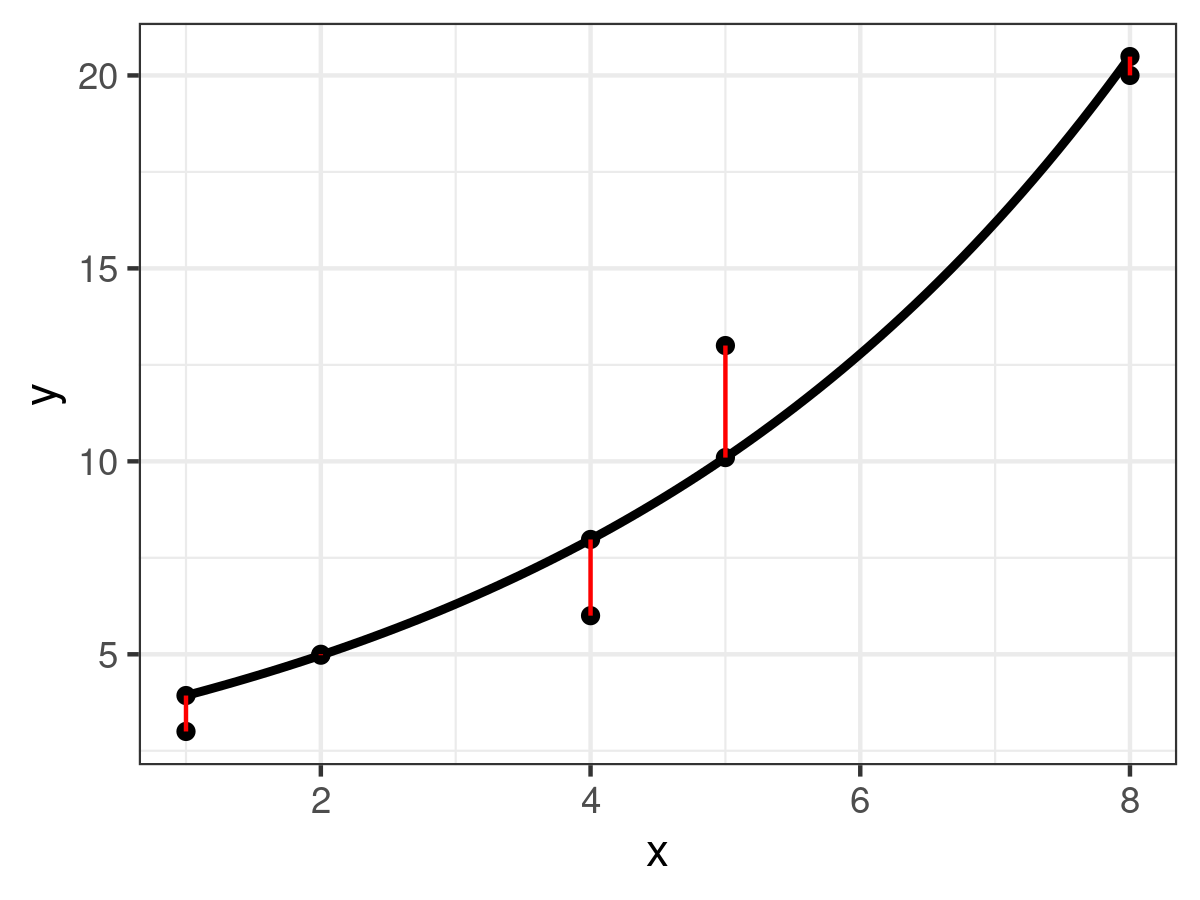
\includegraphics[width=1\textwidth]{figure_man/squares.png}
     \end{center}
\end{column}
\end{columns}


% <<echo = F, out.width = '50%', fig.align='center'>>=
% x = c(1, 2, 4, 5, 8)
% y = c(3, 5, 6, 13, 20)
% mod = nls(y ~ a*exp(b*x), start = list(a = 1, b = 0.2))

% d = data.frame(x = x, y = y, pred = predict(mod))

% plot = ggplot(data = d, aes(x = x, y = y)) + geom_point()
% plot = plot + geom_smooth(method = "nls", formula = y ~ a*exp(b*x),method.args = list(start = c(a = 1, b = 0.2)), se = FALSE, color = "black" )
% plot = plot + geom_point(aes(x = x, y = pred))
% plot = plot + geom_segment(aes(x = x, y = y, xend = x, yend = pred), color = "red")
% plot = plot + theme_bw()
% plot
% @


% Allgemein ist die Modellfunktion beschrieben durch:
% $$
% \bm{y} = f(\bm{x_1},...,\bm{x_n})
% $$
% und hat $p \leq k$ Parameter $\bm{\theta} = (\theta_1,...,\theta_p)$ die nun so bestimmt werden sollen dass die Modellfunktion die tatsächlichen Werte $\bm{y}$ möglichst gut beschreibt.

\framebreak

Suppose we suspect an exponential relationship between $x$ and $y$ 
$$
\fxt = \theta_1 \cdot \exp(\theta_2 \cdot x), \quad \theta_1, \theta_2 \in \R.
$$

% Die Residuen lauten also:
% $$
% r^{(i)}(\bm{\theta}) := y^{(i)} - f(x^{(i)}) = y^{(i)} - \theta_1 exp(\theta_2 x^{(i)})
% $$
% \framebreak

% Sei $|| \cdot ||$ die euklidische Norm. Da bei der KQ-Methode der quadrierte vertikale Abstand zwischen beobachtung $y^{(i)}$ und der Modellfunktion $f(x)$ minimiert wird, können wir das Optimierungsproblem schreiben als:
% \footnotesize
% $$
% \min_{\bm{\theta} \in \R^n} \; g(\bm{\theta}) = \min_{\bm{\theta} \in \R^n} \; \frac{1}{2} ||r(\bm{\theta})||^2 = \min_{\bm{\theta} \in \R^n} \; \frac{1}{2} \sum_{i=1}^{n} (r^{(i)})^2 (\bm{\theta}) =  \min_{\bm{\theta} \in \R^n} \; \frac{1}{2} r(\bm{\theta})^{\top}r(\bm{\theta})
% $$

% Dieses Optimierungsproblem möchten wir nun mit Hilfe des Newton Verfahrens lösen. Hierfür beginnen wir mit der Berechnung der Jakobi- und Hessematrix.


Residuals:
\begin{footnotesize}
$$
r(\bm{\theta}) = \mat{\theta_1 exp(\theta_2 x^{(1)}) - y^{(1)} \\\theta_1 exp(\theta_2 x^{(2)}) - y^{(2)}\\ \theta_1 exp(\theta_2 x^{(3)}) - y^{(3)} \\ \theta_1 exp(\theta_2 x^{(4)}) - y^{(4)} \\ \theta_1 exp(\theta_2 x^{(5)}) - y^{(5)} } = \mat{
\theta_1 exp(1 \theta_2) - 3 \\\theta_1 exp(2 \theta_2) - 7\\ \theta_1 exp(4 \theta_2) - 12 \\ \theta_1 exp(5 \theta_2) - 13 \\ \theta_1 exp(7 \theta_2) - 20
}.
$$
\end{footnotesize}

LS problem:

$$
g(\thetab) =  r(\thetab)^\top r(\thetab) = \sum_{i=1}^{5} \left(\yi - \theta_1 \exp\left(\theta_2 x^{(i)}\right)\right)^2.
$$



\end{vbframe}

\begin{vbframe}{Newton-Raphson Idea}


\textbf{Approach:} Calculate NR update direction by solving:

$$
\nabla^2 g(\bm{\theta}^{[t]}) \bm{d}^{[t]} = - \nabla g(\thetab^{[t]}).
$$

The gradient is calculated by applying the chain rule

$$
	\nabla_\theta g(\thetab) = \nabla_\theta \left[r(\thetab)^\top r(\thetab)\right] = 2 \cdot  \nabla r(\thetab)^\top r(\thetab)
$$

with $\nabla r(\bm{\theta})$ the Jacobian matrix of $r(\cdot)$.

\lz

In our example

\begin{footnotesize}
$$
\nabla r(\thetab) = \mat{\frac{\partial r_1(\theta)}{\partial \theta_1} & \frac{\partial r_1(\theta)}{\partial \theta_2}\\
\frac{\partial r_2(\theta)}{\partial \theta_1} & \frac{\partial r_2(\theta)}{\partial \theta_2}\\
\vdots & \vdots \\
\frac{\partial r_5(\theta)}{\partial \theta_1} & \frac{\partial r_5(\theta)}{\partial \theta_2}} 
= \mat{exp(\theta_2 x^{(1)}) & x^{(1)} \theta_ 1 exp(\theta_2 x^{(1)}) \\ exp(\theta_2 x^{(2)}) & x^{(2)} \theta_ 1 exp(\theta_2 x^{(2)})\\ exp(\theta_2 x^{(3)}) & x^{(3)} \theta_1 exp(\theta_2 x^{(3)}) \\ exp(\theta_2 x^{(4)}) & x^{(4)} \theta_1 exp(\theta_2 x^{(4)}) \\ exp(\theta_2 x^{(5)}) & x^{(5)} \theta_1 exp(\theta_2 x^{(5)})} 
% = \mat{exp(1 \theta_2) & 1 \theta_1 exp(1 \theta_2 ) \\ exp(2 \theta_2) & 2 \theta_1 exp(2 \theta_2 )\\ exp(4 \theta_2) & 4 \theta_1 exp(4 \theta_2) \\ exp(5 \theta_2) & 5 \theta_1 exp(5 \theta_2) \\ exp(7 \theta_2) & 7 \theta_1 exp(7 \theta_2)}
$$
\end{footnotesize}

\framebreak 

Hessian is obtained by applying product rule and has elements

\begin{eqnarray*}
	H_{jk} &=& 2 \sumin \left(\frac{\partial r_i}{\partial \thetab_j}\frac{\partial r_i}{\partial \thetab_k} + r_i \frac{\partial^2 r_i}{\partial \thetab_j \partial \thetab_k}\right)
\end{eqnarray*}

% \begin{eqnarray*}
% \nabla^2_\theta \left(r(\thetab)^\top r(\thetab)\right) &=& \nabla_\theta \left(\nabla_\theta \left(r(\thetab)^\top(\thetab)\right)\right) = \nabla_\theta \left[2 \cdot  \nabla r(\thetab)^\top r(\thetab)\right] \\ 
% &=& 2 \nabla_\theta r(\thetab)^\top \nabla_\theta r(\thetab) + 
% \end{eqnarray*}


% The Hessian matrix $\nabla^{2} f(\bm{\theta})$ is obtained by applying the chain rule:

% % muss eine p x p - Matrix sein
% % r ist ein n x p Vektor
% % nabla r_i ist p x 1
% \begin{align*}
% \nabla^{2} \left(\frac{1}{2}\cdot r(\bm{\theta})^\top r(\bm{\theta}) \right) &= \nabla r(\bm{\theta})^\top \nabla r(\bm{\theta}) + \sum_{i=1}^{n} r^{(i)}(\bm{\theta}) (\nabla^2)^{(i)}(\bm{\theta})
% % &= J(\bm{\theta})^\top J(\bm{\theta}) + W(\bm{\theta})
% \end{align*}

\textbf{Problem with NR:} 2nd derivatives can be challenging to compute! 

\end{vbframe}

\begin{vbframe}{Gauss Newton for least squares}

GN approximates H by dropping its second part:

\begin{eqnarray*}
H_{jk} &=& 2 \sumin \left(\frac{\partial r_i}{\partial \thetab_j}\frac{\partial r_i}{\partial \thetab_k} + r_i \frac{\partial^2 r_i}{\partial \thetab_j \partial \thetab_k}\right) \\
&\approx&  2 \sumin \left(\frac{\partial r_i}{\partial \thetab_j}\frac{\partial r_i}{\partial \thetab_k}\right) = 2 \nabla r^\top \nabla r.  
\end{eqnarray*}

assuming for all $i$ that 
$$
	 \left|\frac{\partial r_i}{\partial \thetab_j}\frac{\partial r_i}{\partial \thetab_k}\right| \gg \left|r_i \frac{\partial^2 r_i}{\partial \thetab_j \partial \thetab_k}\right|.
$$

This assumption may be valid if: 

\begin{itemize}
	\item Residuals $r_i$ are small in magnitude
	\item Functions are only \enquote{mildly} nonlinear and $\frac{\partial^2 r_i}{\partial \thetab_j \partial \thetab_k}$ is small. 
\end{itemize}

\framebreak 

If $\nabla r(\thetab)^\top \nabla r(\thetab)$ is invertible, the Gauss-Newton update direction is 

\begin{eqnarray*}
\bm{d}^{[t]} &=& - \left[\nabla^2 g(\bm{\theta}^{[t]})\right]^{-1} \nabla g(\thetab^{[t]}) \\
&=& - \left[\nabla r(\thetab)^\top \nabla r(\thetab)\right]^{-1} \nabla r(\thetab)^\top r(\thetab),
\end{eqnarray*}

\lz

\textbf{Advantage}: Reduced computational complexity because Hessian does not have to be computed. 


% \textbf{Solution:} Gauss-Newton algorithm
% \begin{itemize}
% \item If residuals $r^{(i)}(\bm{\theta})$ small, approximation of the Hessian matrix:
% \begin{align*}
% \nabla^{2} f(\bm{\theta}) &= \nabla r(\bm{\theta})^\top \nabla r(\bm{\theta}) + \underbrace{\sum_{i=1}^{n} r^{(i)}(\bm{\theta}) \nabla^{2}r^{(i)}(\bm{\theta})}_{\approx 0} \approx \nabla r(\bm{\theta})^{\top} \nabla r(\bm{\theta})
% \end{align*}

% \item Hessian matrix is therefore not explicitly calculated \\ $\rightarrow$ less effort than Newton's method.
% % \item Quadratische Konvergenz bei Startwert nahe des Optimums
% % \item Algorithmus iteriert durch die Parameter $\bm{\theta}$.
% \end{itemize}

% \textbf{Prerequisites for Gauss Newton:}
% \begin{itemize}
% \item Residuals must be sufficiently small so that approximation is not too bad
% % \item initial value of the parameters $\bm{\theta}$ must be sufficiently close to the optimal solution (otherwise procedure does not converge)
% \item Full Rank of the Jacobian matrix $\nabla r(\bm{\theta})$ (so that solution of the LES possible)
% \end{itemize}

% \framebreak

% Instead of using the exact Newton-Raphson search direction

% \begin{eqnarray*}
% \nabla^2 f(\bm{\theta}^{[t]}) \bm{d}^{[t]} &=& - \nabla f(\bm{x}^{[t]}),
% \end{eqnarray*}

% we are using a simplified Newton-Raphson search direction:

% \begin{eqnarray*}
% \nabla r(\bm{\theta}^{[t]})^\top\nabla r(\bm{\theta}^{[t]}) \bm{d}^{[t]} &=& - \nabla  r(\bm{\theta}^{[t]})^\top r(\bm{\theta}^{[t]})
% \end{eqnarray*}

% Dieses Gleichungssystem ist widerum ein überbestimmtes Gleichungssystem, das wir durch die analytische Lösung des Optimierungsproblems

% \begin{eqnarray*}
% \text{arg } \min_{\bm{d}_i} \frac{1}{2} \|\nabla r(\bm{\theta}_i) \bm{d}_i + r(\bm{\theta}_i)\| \\
% \bm{d}_i = \left(\nabla r(\bm{\theta}_i)^\top \nabla r(\bm{\theta}_i)\right)^{-1} \nabla r(\bm{\theta}_i)^\top  \left(r(\bm{\theta}_i\right)
% \end{eqnarray*}

% ersetzen.

% \lz


% $$
% \nabla^{2} g(\bm{\theta}) = J(\bm{\theta})^\top J(\bm{\theta})
% $$

% Die Gauss-Newton-Suchrichtung $\bm{d}_i$ lautet somit

% $$
% \nabla^{2} g(\bm{\theta}) d_{G} = -\nabla g(\bm{\theta})
% $$
% $$
% J(\bm{\theta})^{\top} J(\bm{\theta}) d_{GN} = J(\bm{\theta})^{\top} r(\bm{\theta})
% $$
% \medskip

% Die Iterationsvorschrift des Gauß-Newton Verfahrens lautet:
% $$
% \bm{\theta}_{i+1} = \bm{\theta}_{k} + \bm{d}_{i}
% $$
% wobei $\bm{\delta}_k$ die Lösung des folgenden Optimierungsproblems in der $k$-ten Iterations ist:
% $$
% \min_{d} \; \frac{1}{2} ||J_k d + r_k||^2 = \min_{d} \; \frac{1}{2} ||J_k d -(-r(\bm{\theta}))||^2
% $$
% Die Lösung ist dann durch die Normalengleichung bestimmt:
% $$
% J_{k}^\top J_{k} d = -J_{k}^\top r_k \Leftrightarrow d = (J_{k}^\top J_{k})^{-1} J_{k}^\top(-r_k)
% $$
% \medskip

% Das Minimum entspricht also der Gauß-Newton-Suchrichtung $d_{GN} = d $
% \lz

% \textbf{Note:} In \texttt{R} LS estimators for non-linear relationships can be determined using the \texttt{nls()} function. This function uses the Gauss Newton algorithm by default.

\end{vbframe}
%
% \framebreak
%
% \normalsize
% \textbf{Allgemein: }
%
%
%
% \begin{itemize}
% \item Sei $r$ Funktion eines n-dimensionalen Vektors
%
% \vspace*{-0.2cm}
%
% $$
%   g: \; \R^p \rightarrow \R^n.
% $$
%
% In vorherigem Beispiel bildet die Funktion $g$ den $p$-dimensionalen Parametervektor $\bm{\theta}$ auf die $n$ Residuen ab.
%
% \item \textbf{Ziel}: $g(x)$ so nah wie möglich an Null, z.B. bezüglich quadratischem Abstand
%
% \vspace*{-0.2cm}
% $$
% \min_{x\in\R^p} f(x) = \min_{x\in\R^p} \; \frac{1}{2} ||g(x)||_2^2 = \min_{x\in\R^p} \; \frac{1}{2} \sum_{i=1}^{n} g_i^2(x).
% $$
% \item Kann als elementweise Penalty der Werte von $g(x)$ angesehen werden (auch andere Penalty vorstellbar, z.B. L1-Norm $\min_{x\in\R^p}\; \sum_{i=1}^n |g_i(x)|$).
% \end{itemize}
%
% <<echo=FALSE, fig.align='center'>>=
% int = seq(-2,2,l=300)
% plot(int,  int^2/2, type = "l", xlab = expression(g[i](x)), ylab = "Penalty")
% points(int, abs(int), type="l")
% @
% %
% % \framebreak
% %
% % \begin{itemize}
% % \item Allgemein lässt sich Penalty darstellen als:
% % $$
% % f(x)=\sum_{i=1}^{m} \phi(g_i(x))
% % $$
% % % \lz
% % % \item Dadurch auch auf z.B. Constrained Optimierung übertragbar
% % \end{itemize}
%
% \framebreak
%
% Allgemein lässt sich Penalty darstellen als:
%
% \lz
% $$
% f(x)=\sum_{i=1}^{n} \phi(g_i(x))
% $$
% \lz
%
% \textbf{Ableitungen von $f(x)$}:
% \begin{itemize}
% \lz
% \item $\nabla f(x) = \sum_{i} \phi'(g_i(x)) \nabla g_i(x)$
% \lz
% \item $\nabla^2 f(x) = \sum_{i} [\phi''(g_i(x)) \nabla g_i(x)] \nabla g_i(x)^T + \phi'(g_i(x)) \nabla^2g_i(x)$
% \end{itemize}
% \framebreak
%
% \textbf{Matrixform:}
% \lz
% \begin{itemize}
% \item $\nabla f(x)= \nabla g(x) \phi'(g(x))$
% \lz
% \item $\nabla^2 f(x)= \nabla g(x) \Phi''  \nabla^{\top} g(x) + \sum_i \phi'(g_i(x)) \nabla^2 g_i(x),$
% \end{itemize}
%
% mit
% $$
% \nabla g(x) = [\nabla g_1(x), \nabla g_2(x), \ldots, \nabla g_n(x)] \text{ (Jacobi-Matrix)},
% $$
% $$
% \phi'(g(x)) = [\phi'(g_1(x)), \ldots, \phi'(g_n(x))]^{\top},
% $$
% $$
% \Phi'' = \diag(\phi''(g_1(x)), \ldots, \phi''(g_n(x)))
% $$
%
% \begin{footnotesize}
% Wegen Blockmatrix-Produkt:
% $$
%   [\nabla g_1(x), \ldots, \nabla g_n(x)] \Phi'' [\nabla g_1(x), \ldots, \nabla g_n(x)]^{\top}
%    = \sum_i \Phi'' \nabla g_i(x) \nabla^{\top} g_i(x)
% $$
% \end{footnotesize}
%
% \framebreak
%
% \textbf{Im Least Squares Fall:} \\
% \lz
% \begin{itemize}
% \item Penalty: $\phi(t) = \frac{1}{2} t^2$,  $\phi'(t) =t$, $\phi''(t) =1$, $\Phi''= I$
% \lz
% \item Setze in Formeln von vorheriger Slide ein:
% \begin{itemize}
% \lz
% \item $\nabla f(x) = \nabla g(x) g(x)$
% \lz
% \item $\nabla^2 f(x) = \nabla g(x) \nabla^{\top}g(x) + \sum_{i} g_i(x)\nabla^2 g_i(x)$
% \end{itemize}
% \end{itemize}

% \framebreak
%
%
%
% \textbf{Idee Gauss-Newton Methode:} \\
% \begin{itemize}
% \item Was passiert mit $\nabla^2 f(x)$ wenn nahe an Minimum und damit $g_i$ klein?
% $$
% \nabla^2 f(x)  \approx \nabla g(x) (\nabla g(x))^{\top} = H(x),
% $$
% H(x) positiv (semi-)definit.
%
% \item Gauss-Newton ähnlich Newton Methode:
% $$
% x^{(i+1)} =  x^{(i)} - \lambda H^{-1}(x^{(i)}) \nabla g(x^{(i)}) g(x^{(i)}),
% $$
% mit $\lambda$ Schrittweite und $\nabla g(x^{(i)}) g(x^{(i)})$ Gradient von f an der Stelle $x^{(i)}$.
% \end{itemize}
\begin{vbframe}{Levenberg-Marquardt algorithm}

If $\nabla r(\bm{\theta}^{[t]})^\top\nabla r(\bm{\theta}^{[t]})$ singular, use $\nabla r(\bm{\theta}^{[t]})^\top\nabla r(\bm{\theta}^{[t]})+\Delta$ with $\Delta$ non-negative diagonal matrix.
\lz
$$
\Delta = \epsilon \cdot I
$$
or
$$
\Delta = \epsilon \cdot \diag\left(\nabla r(\bm{\theta}^{[t]})^\top\nabla r(\bm{\theta}^{[t]})\right)
$$

LMA is an efficient and popular method for solving nonlinear optimization problems.

\lz

Note: The diag elements of a pd matrix are always $\geq 0$

\end{vbframe}

\endlecture
\end{document}


